\section{Mathematical Circuits Using the Op. Amp.: part II}

\subsection{Experiment Design}
    \subsubsection{Background}
    Besides basic amplification and basic algebraic operations, the operational amplifier can also be used to perform mathematical operations like differnciation, intergration, logarithm etc. And in this experiment, we will implement four mathematical operations using the operational amplifier.

    \subsubsection{Propose}
    \begin{itemize}
        \item To verify the Op.Amp. circuit for differentiation operation.
        \item To verify the Op.Amp. circuit for integration operation.
        \item To verify the Op.Amp. circuit for logarithm operation.
        \item To verify the Op.Amp. circuit for exponential operation.
    \end{itemize}

\subsection{Experiment Design}
    \subsubsection{Materials}
        In this experiment, we will use the following components:
        \begin{itemize}
            \item Capacitors
            \item 1N4148 Diode
            \item LM741\_1 Op.Amp.
            \item Resistors
            \item Breadboard
            \item DC power supply
            \item Digital Multi-Meter
            \item Oscilloscope
            \item Function Generator
        \end{itemize}

    \subsubsection{Circuit Diagram}
        The following circuit diagrams shows the Op.Amp. circuits for differentiation, integration, logarithm and exponential operations.
        \begin{figure}[H]
            \centering
            \begin{subfigure}{0.4\textwidth}
                \includegraphics[width=1\linewidth]{Experiment_11/Circuit/Lab11a.drawio.png}
                \caption{Circuit of Differentiation}
                \label{cir:diff}
            \end{subfigure}
            \begin{subfigure}{0.4\textwidth}
                \includegraphics[width=1\linewidth]{Experiment_11/Circuit/Lab11b.drawio.png}
                \caption{Circuit of Integration}
                \label{cir:int}
            \end{subfigure}

            \begin{subfigure}{0.4\textwidth}
                \includegraphics[width=1\linewidth]{Experiment_11/Circuit/Lab11c.drawio.png}
                \caption{Circuit of Logarithm}
                \label{cir:log}
            \end{subfigure}
            \begin{subfigure}{0.4\textwidth}
                \includegraphics[width=1\linewidth]{Experiment_11/Circuit/Lab11d.drawio.png}
                \caption{Circuit of Exponential}
                \label{cir:exp}
            \end{subfigure}
            \caption{Op.Amp. Circuits for Mathematical Operations}
        \end{figure}

    \subsubsection{Theoretical Analysis}
        \begin{enumerate}
            \item \textbf{Differentiation Operation}\newline
                From the figure \ref{cir:diff}, 
                we can see the feedback is through a resistor, and the input voltage is connct to the negetive terminal of the Op.Amp. through a capacitor. 
                So we conclude that this circuit is a differentiator circuit. The output voltage of the circuit is given by:
                \begin{equation}
                    V_{out} = -RC\frac{dV_{in}}{dt}
                \end{equation}
                Where in our circuit, the $R = 1M \Omega$ and $C = 0.1\mu F$.
                \newline

            \item \textbf{Integration Operation}\newline
                From the figure \ref{cir:int}, 
                we can see the feedback is through a parallel conncetion of a resistor and a capacitor, and the input voltage is connct to the negetive terminal of the Op.Amp. through a resistor.
                So we can see it's an integrator circuit. The output voltage of the circuit is given by:
                \begin{equation}
                    V_{out} = -\frac{1}{RC}\int V_{in}dt
                \end{equation}
                Where in our circuit, the $R = 10k \Omega$ and $C = 0.1\mu F$.
                \newline

            \item \textbf{Logarithm Operation}\newline
                From the figure \ref{cir:log}, one may notice the feedback is through a dioide, and the input voltage is connct to the negetive terminal of the Op.Amp. through a resistor.
                So we can see this is logarithm circuit. The output voltage of the circuit is given by:
                \begin{equation}
                    V_{out} = -\frac{R_2}{R_1}ln\left(\frac{V_{in}}{V_{ref}}\right)
                \end{equation}
                Where in our circuit, the $V_{ref}$ is the amplitude of the reference voltage, and $R_1 = R_2 = 100k \Omega$.
                \newline
            \item \textbf{Exponential Operation}\newline
                From the figure \ref{cir:exp}, we notice the feedback is through a resistor, and the input voltage is connct to the negetive terminal of the Op.Amp. through a dioide.
                So we know this circuit is an exponential circuit. The output voltage of the circuit is given by:
                \begin{equation}
                    V_{out} = V_{ref}e^{V_{in}}
                    \label{eq:exp}
                \end{equation}
                Where in our circuit, the $V_{ref}$ is the reference voltage.
        \end{enumerate}

\subsection{Experiment record}
    \subsubsection{The intergration operation circuit}
    \begin{enumerate}[I]

        \item \textbf{Data Recorded}\newline
            The recorded data for the differentiation operation circuit is shown in the table \ref{tab:diff}.
            % Table generated by Excel2LaTeX from sheet 'Sheet1'
            \begin{table}[H]
                \centering
                \begin{tabular}{l|rrrrr}
                    Frequency ($Hz$) & 200.00  & 400.00  & 600.00  & 800.00  & 1000.00  \\
                    \midrule
                    Ampititude ($mV$) & 1800  & 2900  & 4200  & 5450  & 6650  \\
                    Phase ($^\circ$) & 94.56  & 94.40  & 91.53  & 96.43  & 97.49  \\
                \end{tabular}%
                \caption{Data Recorded for Differentiation Operation}
                \label{tab:diff}
            \end{table}
            In addition, here is the plot of the output voltage versus the input voltage for the circuit when connect to a square wave signal.
            \begin{figure}[H]
                \centering
                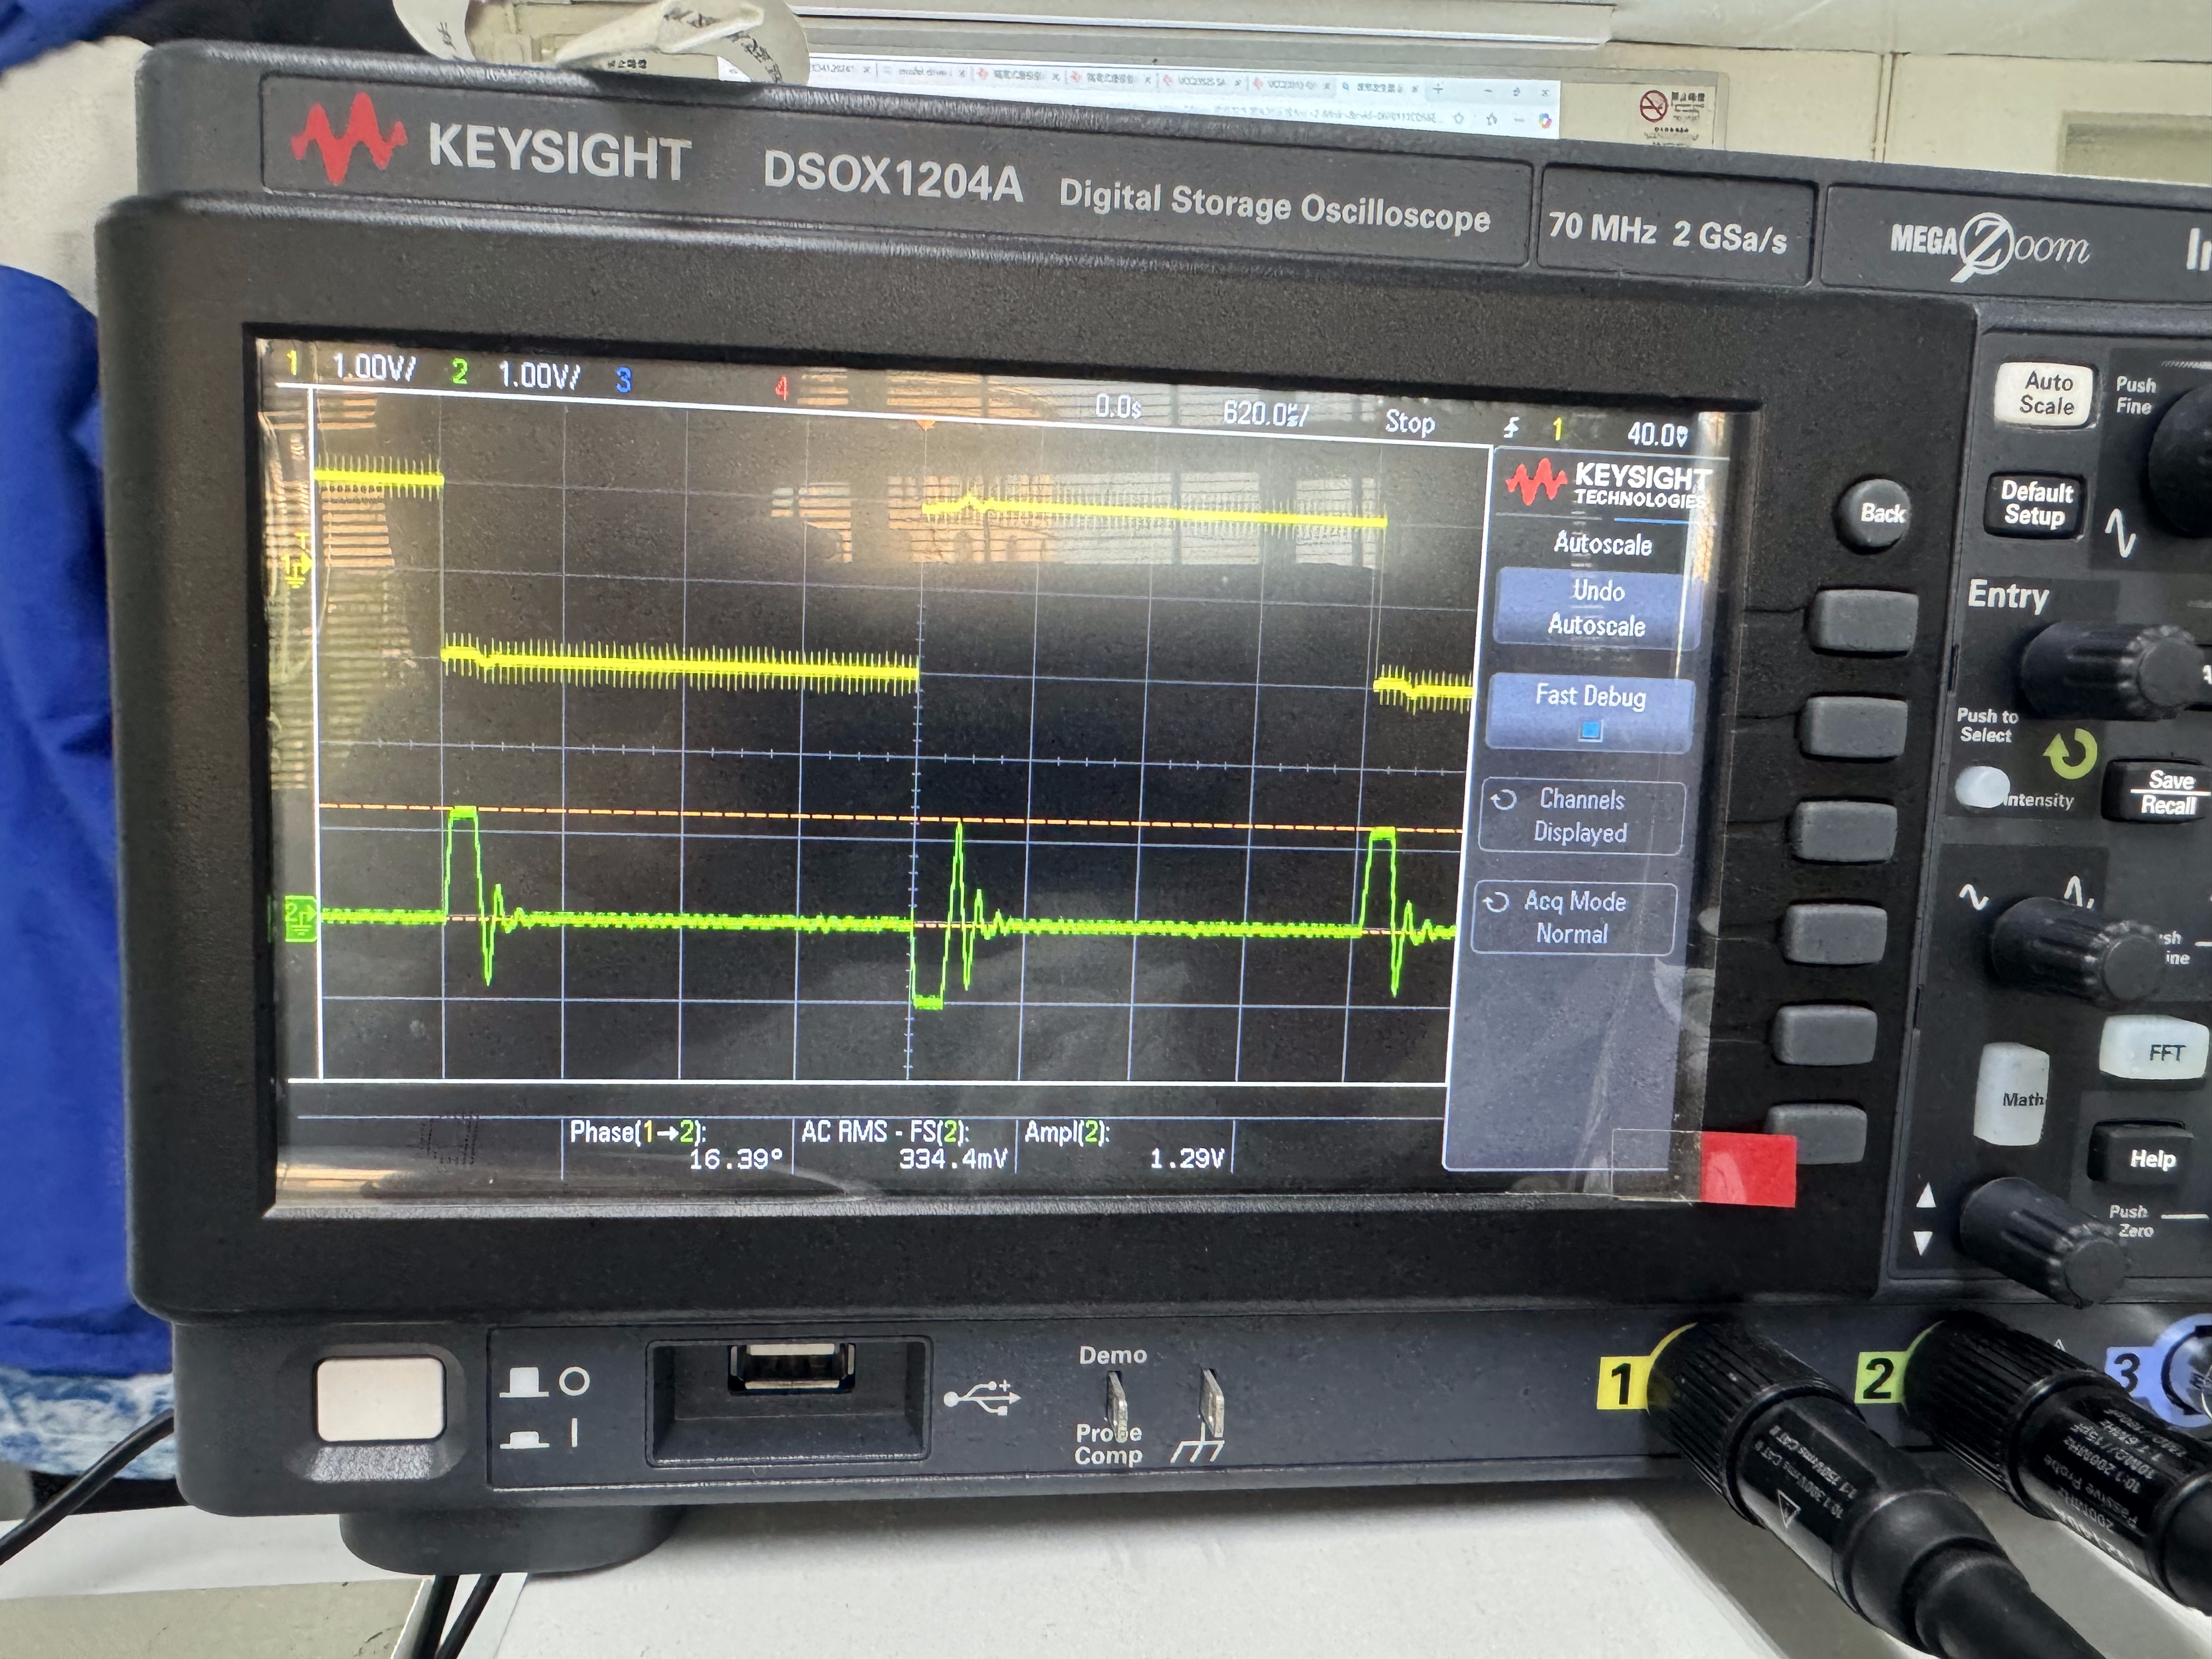
\includegraphics[width=0.6\linewidth]{Experiment_11/Images/cir1_squar.jpg}
                \caption{Output waveform with square wave signal input}
                \label{wave:diff}
            \end{figure}

        \item \textbf{Data Analysis}\newline
            From the output table \ref{tab:diff}, we can see as the Frequency of the input signal increase, the amplitude and the phase difference between input and output increase.\par 
            
            This is beacuse as the frequency increase, the rate of change of the input signal also increase, thus we have a higher amplitude as output, as the output is giving by 
                \begin{equation*}
                    V_{out} = -RC\frac{dV_{in}}{dt}
                \end{equation*}
            \par

            And the phase difference increases because circuit is not ideal, and have a higher phase shifts at higher frequencies.\par

            Finally, with respect to the output wave form in figure \ref{wave:diff}. This is because the rate of change of the square wave is approximately infinite at its edges, so the output is a spike at the edges of the square wave.
    \end{enumerate}

    \subsubsection{The intergration operation circuit}
    \begin{enumerate}
        \item \textbf{Data Recorded}\newline
            The recorded data for the integration operation circuit is shown in the table \ref{tab:int}.

            \begin{table}[H]
            % Table generated by Excel2LaTeX from sheet 'Sheet1'
                \centering
                \begin{tabular}{l|rrrr}
                Frequency $Hz$ & 50.00  & 100.00  & 150.00  & 200.00  \\
                \midrule
                Ampititude $V$ & 1.850  & 0.935  & 0.615  & 0.470  \\
                Phase $^\circ$ & -104.16 & -93.47 & -89.7 & -89.83 \\
                \end{tabular}%
                \caption{Data Recorded for Integration Operation}
                \label{tab:int}
            \end{table}

            In addition, this is the plot of the output voltage versus the input voltage for the circuit when connect to a square wave signal.
            \begin{figure}[H]
                \centering
                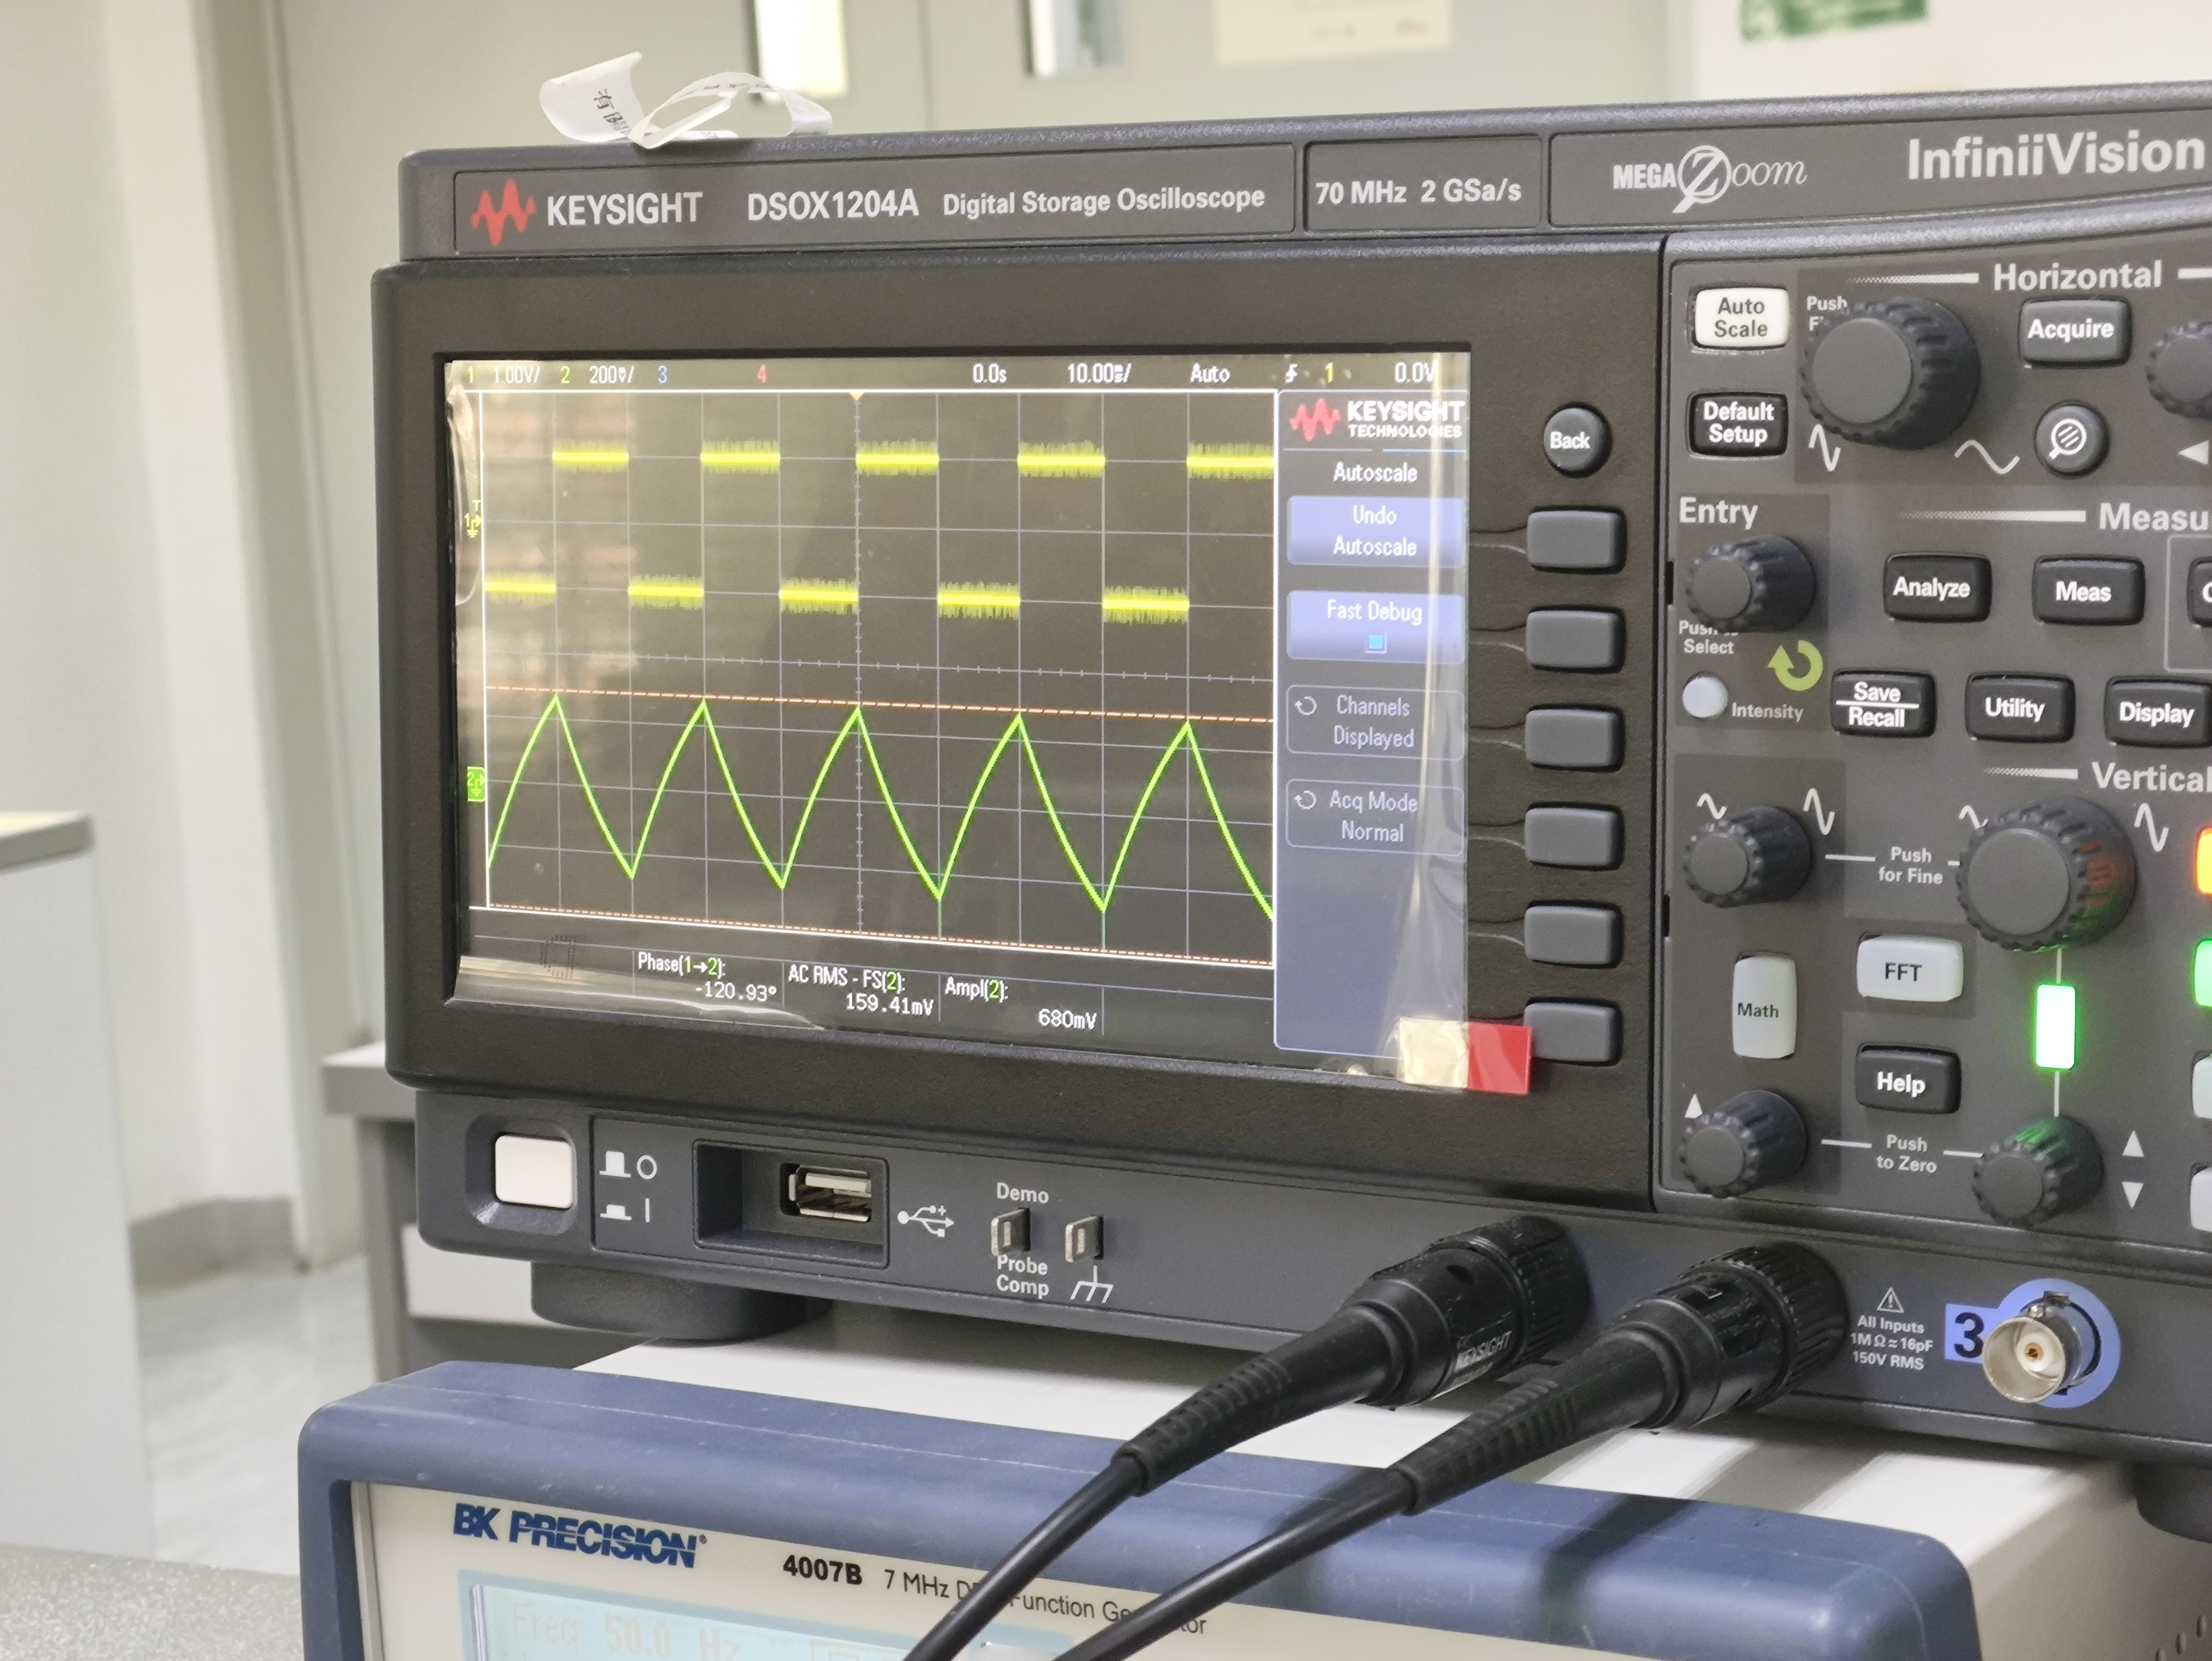
\includegraphics[width=0.6\linewidth]{Experiment_11/Images/cir2_squar.jpg}
                \caption{Output waveform with square wave signal input}
                \label{wave:int}
            \end{figure}

            From the table \ref{tab:int}, we can see as the Frequency of the input signal increase, the amplitude of output decrease. And the phase difference is not in ideal 90$^\circ$, but approching to 90$^\circ$ as frequency increase.\par
        \item \textbf{Data Analysis}\newline
            The amplitude of the output decreases because at higher frequencies, the input signal oscillates faster, and its area (integral) over each cycle becomes smaller. So the output voltage have a smaller amplitude.\par

            The phase difference is negetive because the output is lagging behind the input signal for $\frac{\pi}{2}$. And when the frequency is low, the capacitor reduce the speed of responds, and causing a non perfect phase difference. However, as the frequency increase, the capacitor behave more like a ideal conducter, and the phase difference approching to our expected value.\par

            Finally, with respect to the output wave form in figure \ref{wave:int}. This is because the output is the integral of the input signal, so the output is a triangle wave.
    \end{enumerate}

    \subsubsection{The logarithm operation circuit}
    \begin{enumerate}
        \item \textbf{Data Recorded}\newline
            When the input signal is a triangular wave, the output signal and the input signal is record by the Oscilloscope, and the plot is shown in the figure \ref{wave:log}.
            \begin{figure}[H]
                \centering
                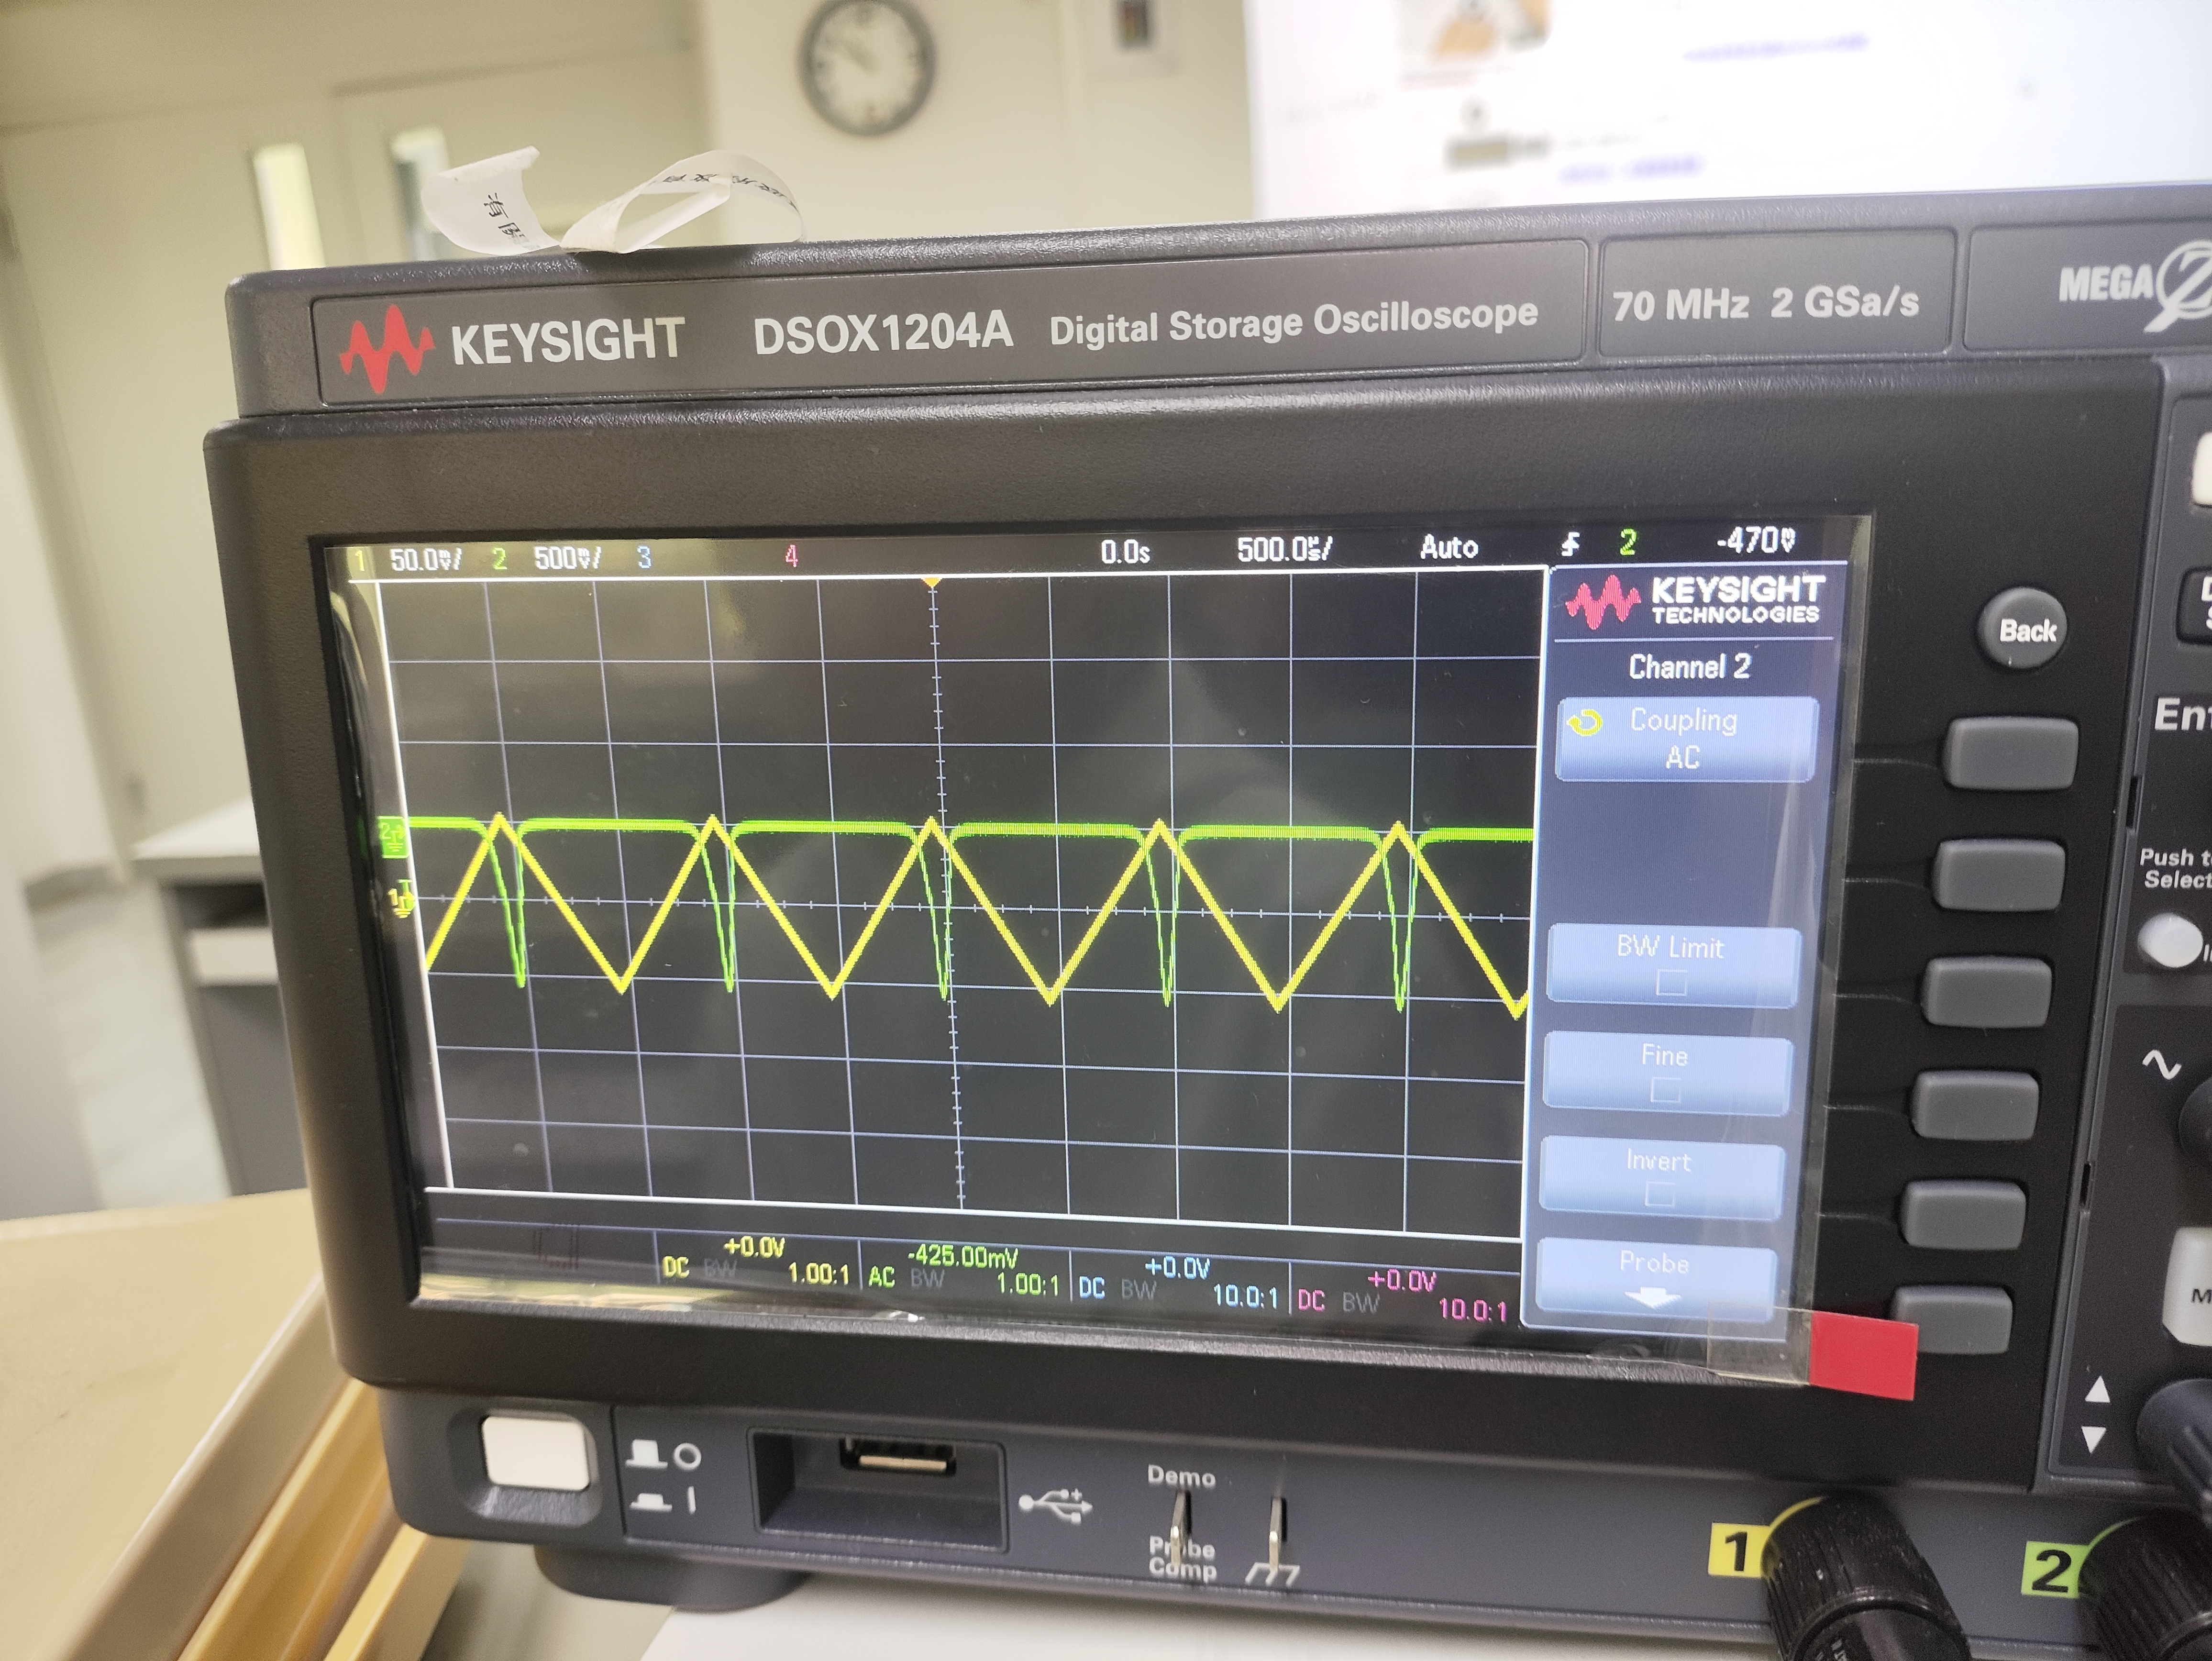
\includegraphics[width=0.6\linewidth]{Experiment_11/Images/cir3_tri.jpg}
                \caption{Output waveform of log circuit with triangular wave signal input}
                \label{wave:log}
            \end{figure}
        \item \textbf{Data Analysis}\newline
            From the ouput wave form in figure \ref{wave:log}, we can see the the output signal is always at zero, around the positive peak of the input signal, the output signal drop to negetive very quickly, and recover to zero quickly when the input signal drop after its peak.\par

            This is because the logarithmic function changes very slowly except near rapid transitions so the output remains close to zero during most of the input. And therefore, at the peak of the input signal, the signal change rapidly, so the output will quickly goes to a extream value quickly. Howver, when the signal approch to the negetive edge, the diode at the feedback loop block the output signal from change to a positive peak, so the ouput looks like what we saw.\par
    \end{enumerate}

    \subsubsection{The exponential operation circuit}
    \begin{enumerate}
        \item \textbf{Data Recorded}\newline
            When the input signal is a triangular wave, the output signal and the input signal is record by the Oscilloscope, and the plot is shown in the figure \ref{wave:exp}.
            \begin{figure}[H]
                \centering
                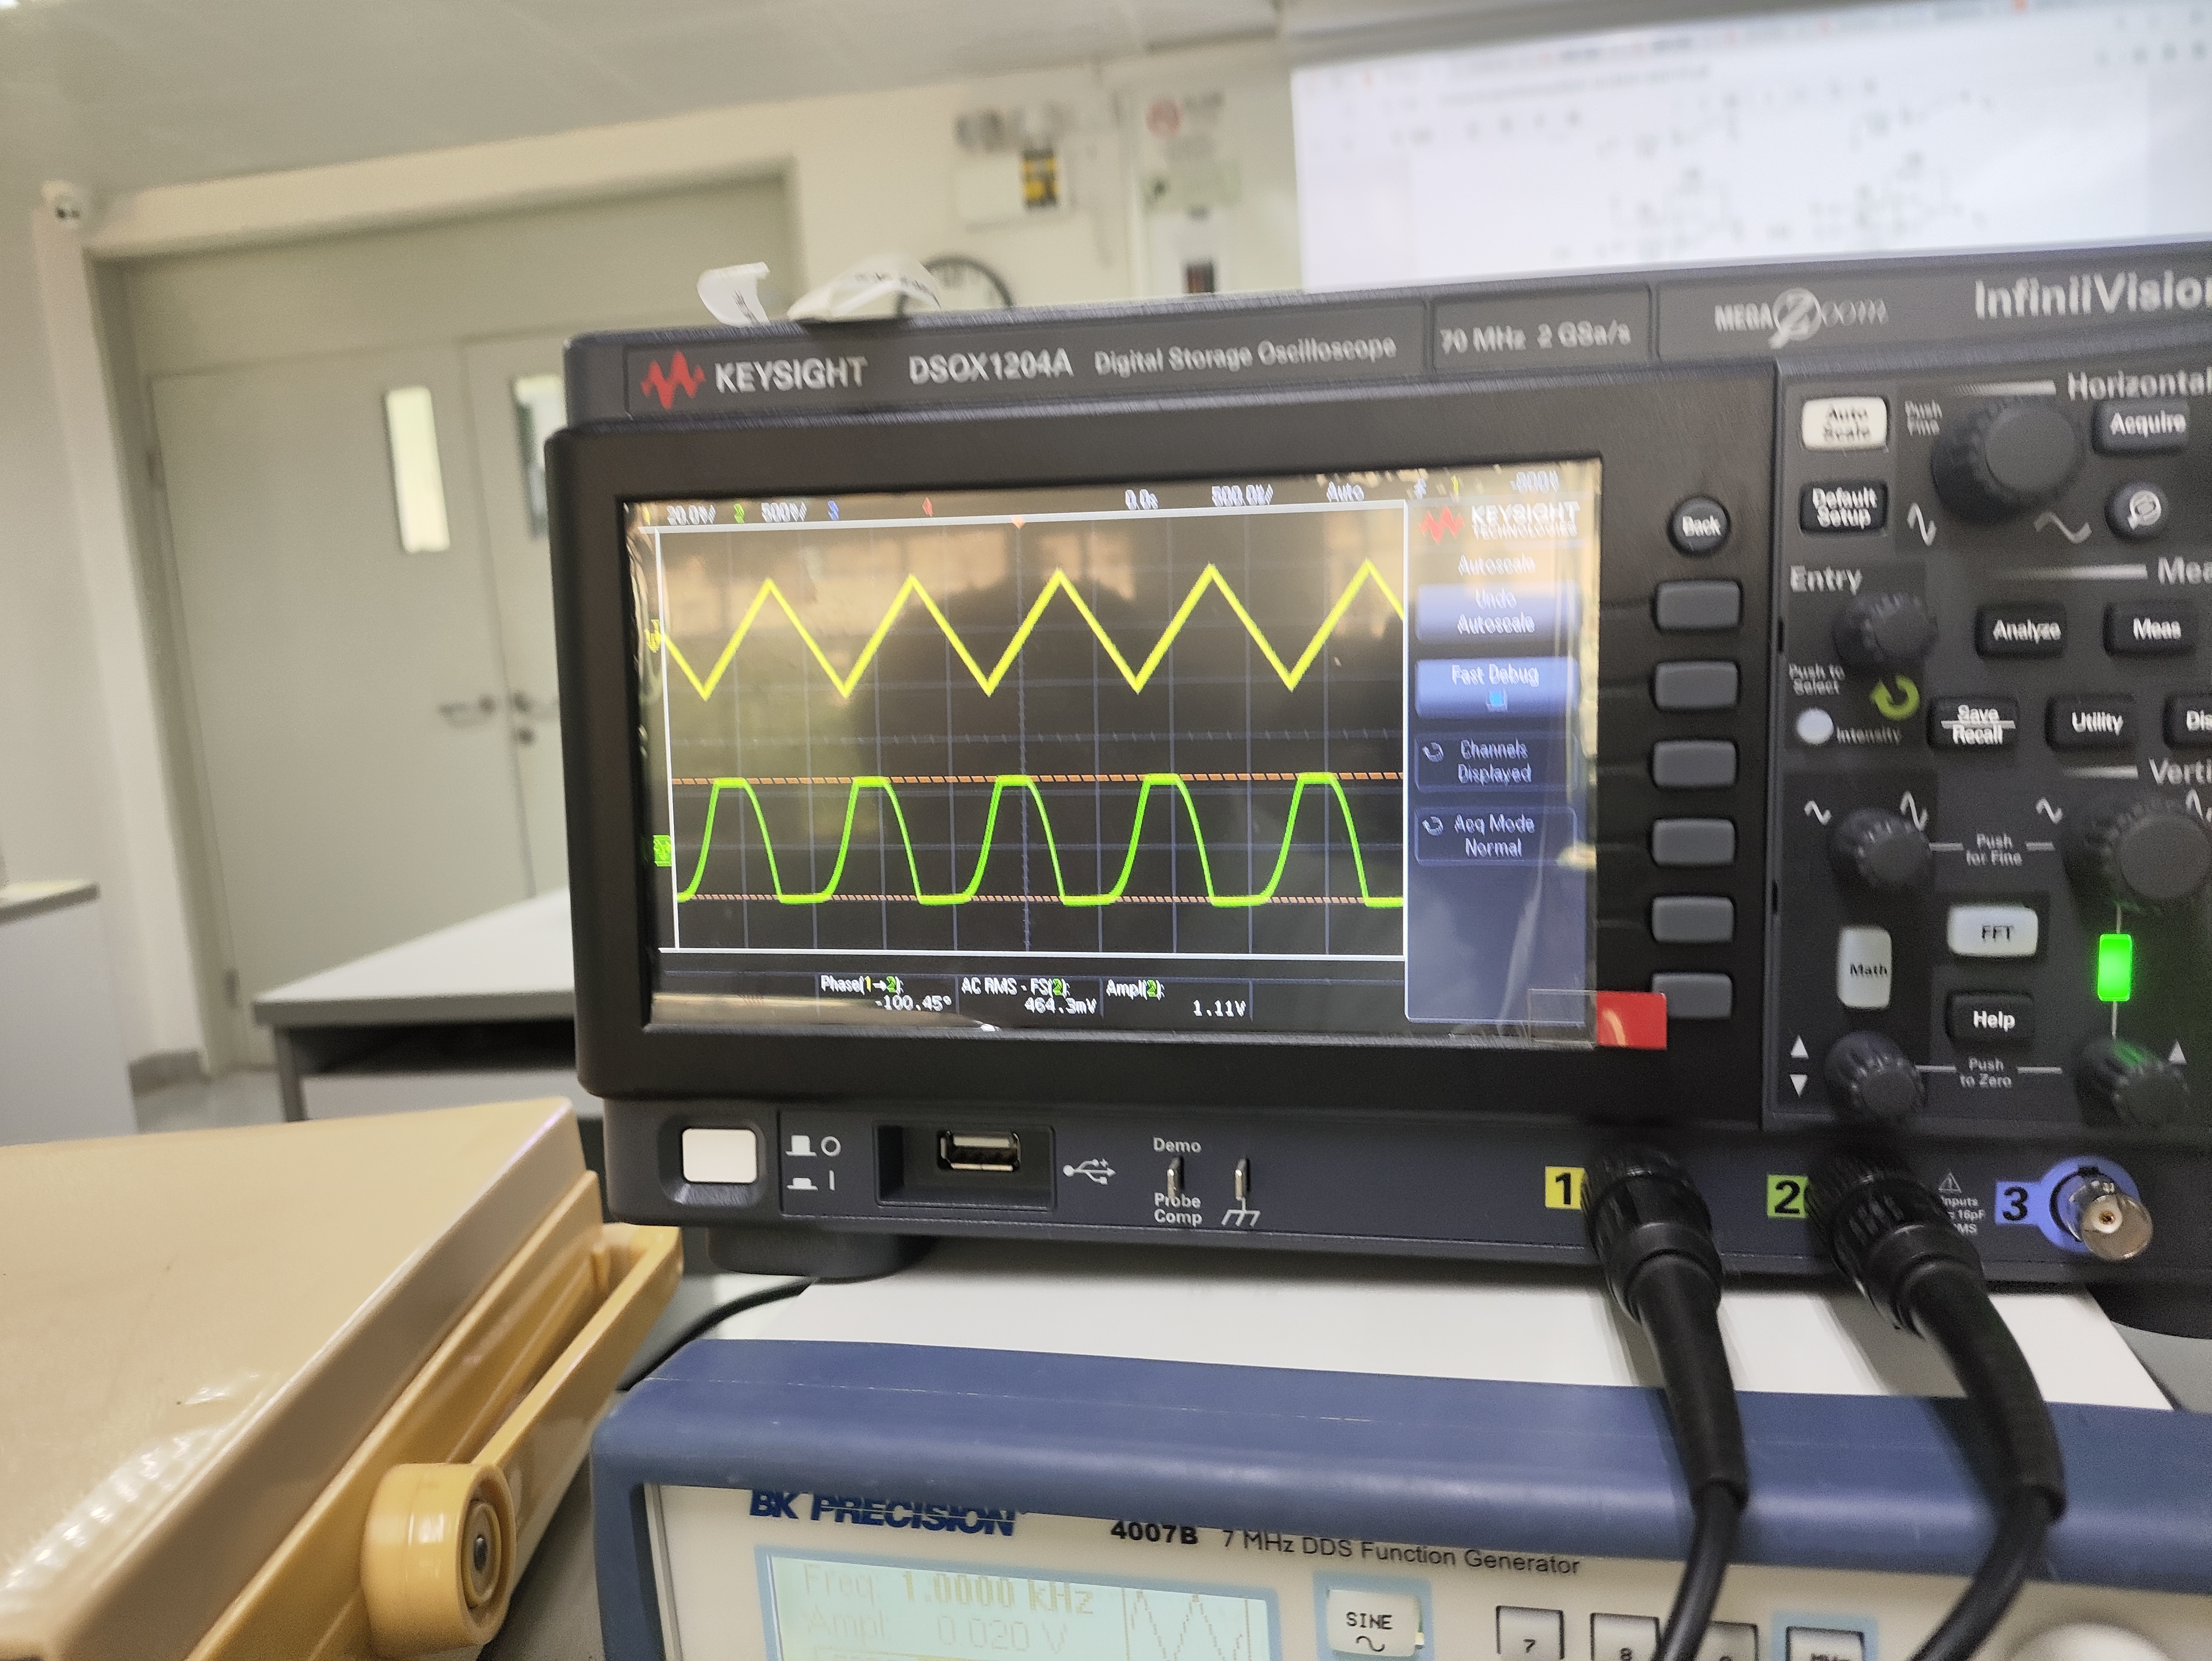
\includegraphics[width=0.6\linewidth]{Experiment_11/Images/cir4_tri.jpg}
                \caption{Output waveform of exponential circuit with triangular wave signal input}
                \label{wave:exp}
            \end{figure}
        \item \textbf{Data Analysis}\newline
            From the output wave form in figure \ref{wave:exp}, we can see at the increase ramp, the output voltage drop in the exponential curve, and at the decrease ramp, the output voltage rise in the exponential curve.\par

            Beacuse the characteristic of the circuit, the output signal behave inversely to the input signal. And due to the exponential nature of the circuit, the output signal is exponential to the input signal as the output signal euqation eq.\ref{eq:exp} shows.\par
    \end{enumerate}

\subsection{Experiment Conclusion}
    \subsubsection{Conclusion}
        In this experiment, we have implemented four mathematical operations using the operational amplifier, and we have verified the circuit for differentiation, integration, logarithm and exponential operations. And we have also analyzed the output wave form of the circuit when connect to different input signals.\par